%Kaptitel 1

\chapter{Aufgabe D2}

\section{Berechnung der Radien}
Im folgenden werden die in der Aufgabenstellung gegebenen Gleichungen verwendet, um die Kurvenradien der einzelnen Räder zu berechnen.\\

	Mit (6) folgt: $ \frac{R_{RR}}{R_{RL}} = \frac{V_{RR}}{V_{RL}}$  \\
	\indent\indent ${R_{RL} = {R_{RR}} * \frac{V_{RR}}{V_{RL}}}$ \\
	Mit (1) folgt: ${R_{RL}} = \frac{V_{RR}}{V_{RL}} * (W+{R_{RL}})$ \\
	\indent\indent ${R_{RL}}-\frac{V_{RR}}{V_{RL}}*{R_{RL}} = \frac{V_{RR}}{V_{RL}} * W$ \\
	\indent\indent ${R_{RL}}*(1-\frac{V_{RR}}{V_{RL}})= \frac{V_{RR}}{V_{RL}} * W$ \\
	\indent\indent ${R_{RL}}= \frac{\frac{V_{RR}}{V_{RL}} * W}{1-\frac{V_{RR}}{V_{RL}}}$ \\
	\indent\indent ${R_{RL}}= \frac{W}{\frac{V_{RR}}{V_{RL}}-1}$ \\
	Mit (1) folgt: ${R_{RR}}= W + {R_{RL}} = W + \frac{W}{\frac{V_{RR}}{V_{RL}}-1}$ \\
	Mit (2) folgt: ${R_{FR}}^2= B^2 + (W + \frac{W}{\frac{V_{RR}}{V_{RL}}-1})^2$ \\
	\indent\indent ${R_{FR}} = \sqrt{B^2 + (W + \frac{W}{\frac{V_{RR}}{V_{RL}}-1})^2}$ \\
	Mit (3) folgt: ${R_{FR}}^2= B^2 + (\frac{W}{\frac{V_{RR}}{V_{RL}}-1})^2$\\
\indent\indent ${R_{FR}} = \sqrt{B^2 + (\frac{W}{\frac{V_{RR}}{V_{RL}}-1})^2}$\\ 

Die erstellten Gleichungen stellen die Grundlage für die folgenden Analysen dar.
\newpage
\section{Analyse der ausgewählten Situationen}
	Im Folgenden wird anhand einiger Graphiken das Verhalten bei Kurvenfahrten analysiert.
	
	In der nachfolgenden \autoref{fig:velo_ohneRand} werden zuerst die Geschwindigkeiten der vier Räder des Fahrzeugs dargestellt. Es ist erkennbar, dass es Abweichungen zwischen den Geschwindigkeiten gibt. Diese werden nachfolgend genauer erläutern.
	\begin{figure}[h!]
		\centering
		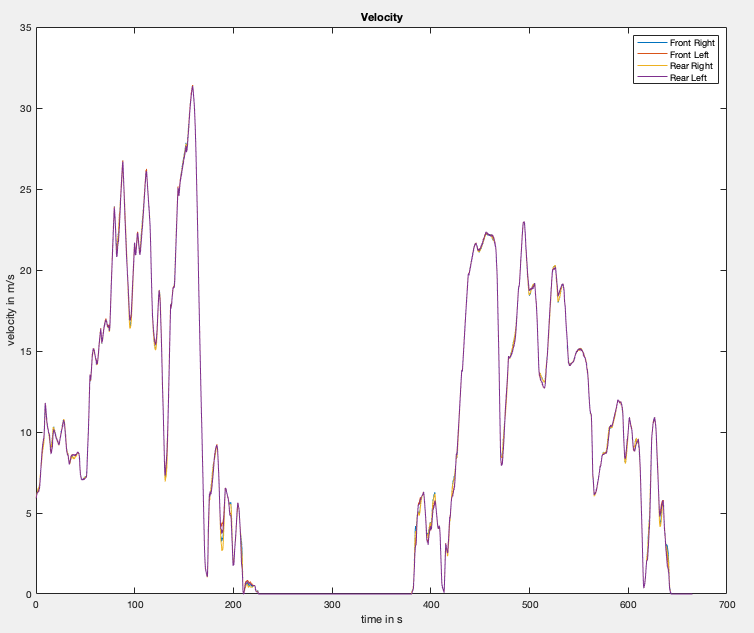
\includegraphics[width=1\linewidth]{../Graphiken/velo_ohneRand}
		\caption{Übersicht der Geschwindigkeiten der vier Räder}
		\label{fig:velo_ohneRand}
	\end{figure}
\pagebreak
%figure('NumberTitle','off','Name','Velocity')
%plot(tv,vfr);
%hold on;
%plot(tv,vfl);
%plot(tv,vrr);
%plot(tv,vrl);
%xlabel('velocity in m/s'); 
%ylabel('time in s');
%legend('Front Right', 'Front Left', 'Rear Right', 'Rear Left');
%title('Velocity');

	%\begin{figure}[h!]
	%	\centering
	%	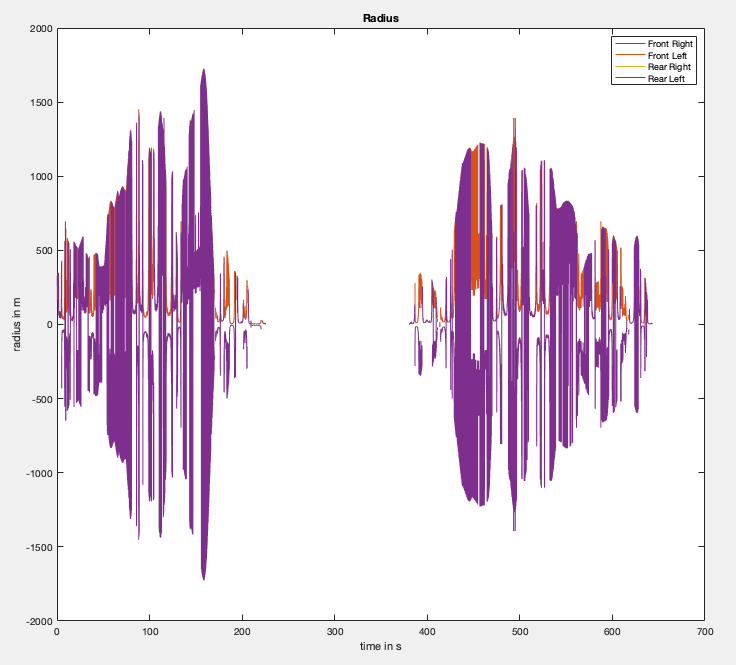
\includegraphics[width=1\linewidth]{../Graphiken/radius}
	%	\caption{Übersicht den Radius der vier Räder}
	%	\label{fig:radius}
	%\end{figure}
% %Alle Radien in einem Plot
% figure('NumberTitle','off','Name','Radius')
% plot(tv,rfr);
% title('Radius');
% hold on;
% plot(tv,rfl);
% plot(tv,rrr);
% plot(tv,rrl);
% xlabel('time in s');
% ylabel('radius in m')
% legend('Front Right', 'Front Left', 'Rear Right', 'Rear Left');

	Die \autoref{fig:velo_vs_sw} zeigt einen Ausschnitt zwischen 495s und 550s. Die Abbildung wurde in einzelne Abschnitte zur Analyse unterteilt. Im ersten Abschnitt, vor 500ms, ist der Lenkradwinkel sehr klein. Man sieht dort kaum keinen Unterschied zwischen den Geschwindigkeiten der linken und rechten Rädern. Im zweiten Abschnitt ist der Lenkwinkel wesentlich höher. Das hat zur Folge, dass die Geschwindigkeit der rechten Räder über der Geschwindigkeit der linken Räder liegt. Beim Wechel vom zweiten in den dritten Abschnitt ist der Winkel kurz Null und steigt dann wieder. Dort liegt die Geschwindigkeit der linken Räder über der Geschwindigkeit der rechten Räder. Daraus lässt sich schließen, dass sich die Fahrt von einer Links- in eine Rechtskurve ändert. Im vorletzen Abschnitt ist wieder eine Linkskurve erkennbar. Im letzten Abschnitt wird kaum gelenkt, aus diesem Grund weichen die Geschwindigkeiten nur sehr gering voneinander ab.
	\begin{figure}[h!]
		\centering
		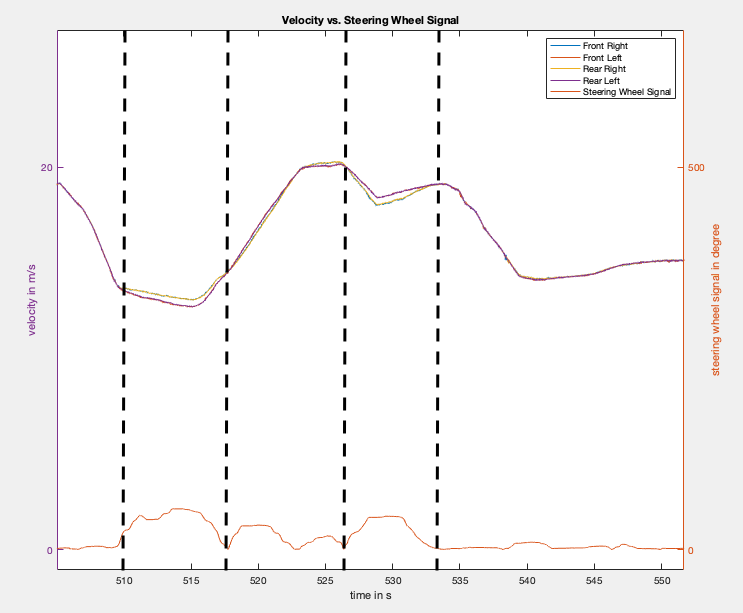
\includegraphics[width=1\linewidth]{../Graphiken/velo_vs_sw}
		\caption{Übersicht der Geschwindigkeiten mit Drehwinkel des Lenkrads}
		\label{fig:velo_vs_sw}
	\end{figure}
%%Alle Geschwindigkeiten in einem Plot
%figure('NumberTitle','off','Name','Velocity')
%plot(tv,vfr);
%hold on;
%plot(tv,vfl);
%plot(tv,vrr);
%[hAx,hLine1,hLine2] = plotyy(tv,vrl,tv,sw);
%xlabel('time in s'); 
%ylabel(hAx(1),'velocity in m/s');
%ylabel(hAx(2),'steering wheel signal in degree');
%legend('Front Right', 'Front Left', 'Rear Right', 'Rear Left', 'Steering Wheel Signal');
%title('Velocity vs. Steering Wheel Signal');
%für zusätzlichen Drehwinkel --> Links oder Rechtsfahrt
\newpage
	Die \autoref{fig:outter_vs_inner} zeigt den Ausschnitt von ca. 510ms bis 517ms. Dieser entspricht dem dem zweiten Abschnitt der \autoref{fig:velo_vs_sw}. Hier werden die Radien der beiden Vorderräder verglichen. Es ist erkennbar, dass der Radius des Rechten Vorderrads immer über dem Radius des Linken liegt. Dies zeigt nochmal, dass es sich hier um eine Linkskurve handelt.
	\begin{figure}[h!]
		\centering
		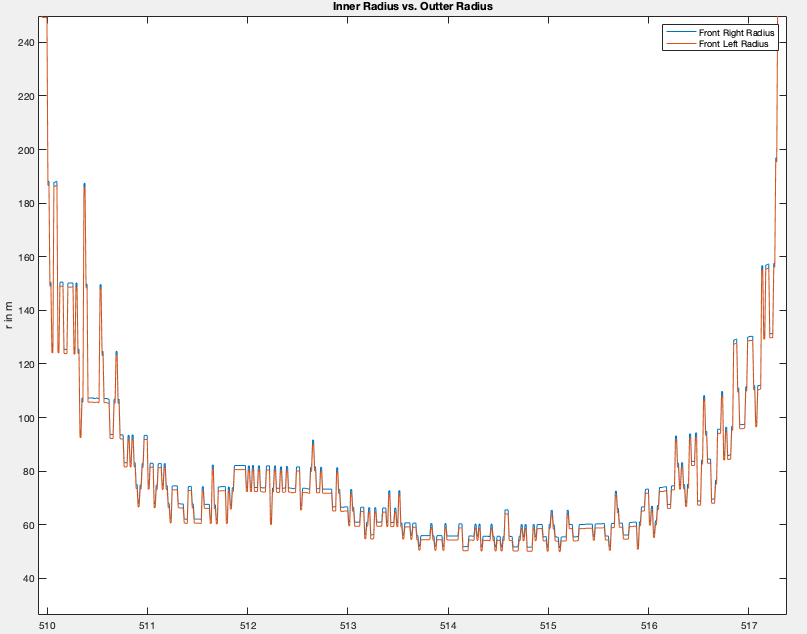
\includegraphics[width=1\linewidth]{../Graphiken/outter_vs_inner}
		\caption{Vergleich des linken und rechten Radius bei Kurvenfahrt}
		\label{fig:outter_vs_inner}
	\end{figure}
\cleardoublepage
\newpage
% %Vorderer Innerer Radius gegen Äußeren Radius
% figure('NumberTitle','off','Name','Inner Radius vs. Outter Radius')
% plot(tv,rfr);
% hold on;
% plot(tv,rfl);
% xlabel('lateral acceleration in g')
% ylabel('r in m');
% legend('Front Right Radius','Front Left Radius')
% title('Inner Radius vs. Outter Radius');


	In der nächsten \autoref{fig:sorted_sw} wird der Radius in Abhängigkeit des Drehwinkels abgebildet. Es zeigt, dass mit steigendem Drehwinkel der Radius immer kleiner wird. Stellen, an denen das Fahrzeug nicht fährt, können hierbei vernachlässigt werden. Allgemein gilt, dass bei Kurvenfahrten der Radradius abnimmt.
	
		\begin{figure}[h!]
		\centering
		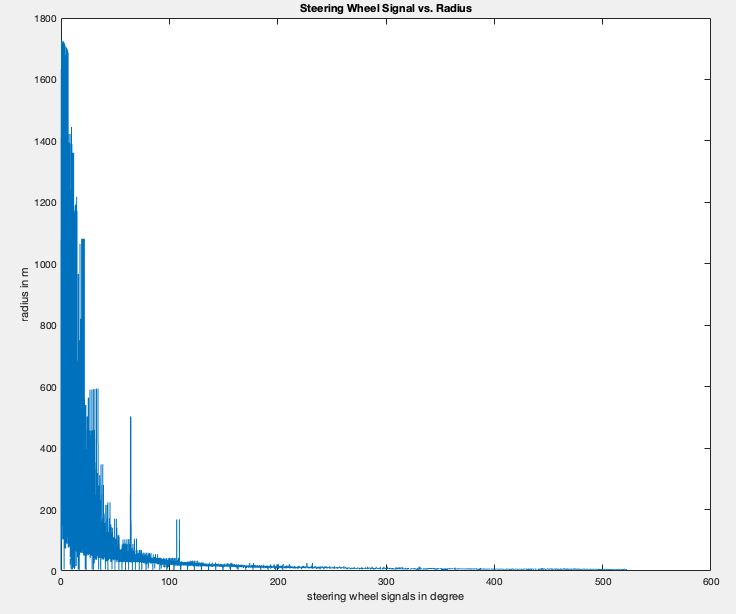
\includegraphics[width=1\linewidth]{../Graphiken/sorted_sw}
		\caption{Lenkraddrehwinkel gegenüber Radius}
		\label{fig:sorted_sw}
	\end{figure}
\pagebreak
% %Sortiertes sw gegen Radius
% figure('NumberTitle','off','Name','Steering Wheel Signal vs. Radius')
% plot(sw_sorted,newrfl);
% xlabel('steering wheel signals in degree');
% ylabel('radius in m');
% title('Steering Wheel Signal vs. Radius');
% %Sortiertes q gegen Radius
% [q_sorted, q_order] = sort(new_q);
% nrfl = rfl(q_order,:);
% figure('NumberTitle','off','Name','Sorted Lateral Acceleration vs. Radius')
% plot(q_sorted,nrfl);
% xlabel('sorted lateral acceleration in g');
% ylabel('radius in m');
% title('Sorted Lateral Acceleration vs. Radius');	

	In der folgenden \autoref{fig:v_vs_r} wird der Radius in Abhängigkeit der Geschwindigkeit dargestellt. Es zeigt, dass bei gleichem Drehwinkel des Lenkrads bei steigender Geschwindigkeit der Radius immer größer wird. 
	\begin{figure}[h!]
		\centering
		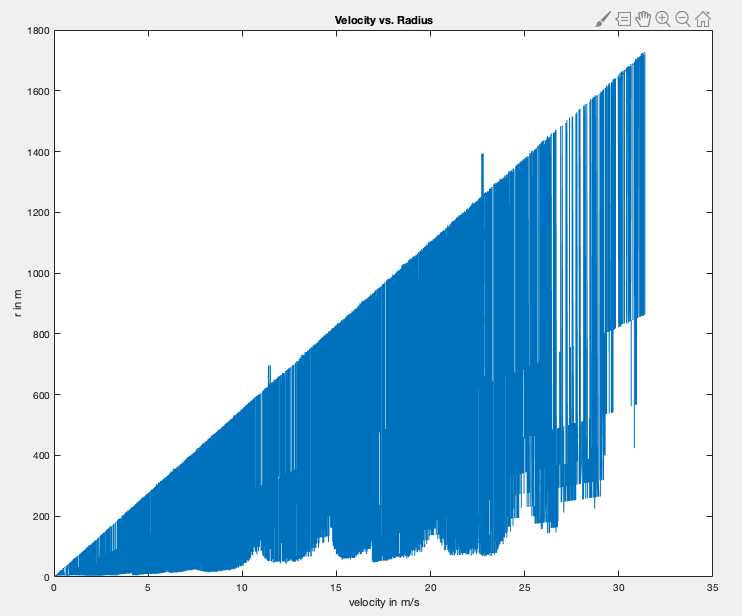
\includegraphics[width=1\linewidth]{../Graphiken/v_vs_r}
		\caption{Geschwindigkeit gegenüber Radius}
		\label{fig:v_vs_r}
	\end{figure}
% %Geschwindigkeit vs Radius SORTIERT
% [v_sorted, v_order] = sort(vfl);
% newradius= rfl(v_order,:);
% figure('NumberTitle','off','Name','Velocity vs. Radius')
% plot(v_sorted,newradius);
% %hold on;
% %plot(tv,rfl);
% xlabel('velocity in m/s')
% ylabel('r in m');
% %legend('Front Right Radius','Front Left Radius')
% title('Velocity vs. Radius');



	
	

	
	
	
	